\section{Законы сохранения момента импульса и энергии}

\introProblems

\begin{ex} %Сив337
Однородный тонкий тяжелый стержень длины $l$ висит на горизонтальной оси, проходящей через один из его концов. Какую начальную угловую скорость и надо сообщить стержню, чтобы он повернулся на $90^{\circ}$?
\begin{ans}
$\omega = \sqrt{3g/l}$.
\end{ans}
\end{ex}	

\begin{ex} %Сив340
На краю свободно вращающегося достаточно большого горизонтального диска, имеющего радиус $R$ и момент инерции $I$, стоит человек массы $m$. Диск совершает $\nu$ об/мин. Как изменится скорость вращения диска, если человек перейдет от края диска к центру? Как изменится при этом энергия системы? Размерами человека по сравнению с радиусом диска можно пренебречь.
\begin{ans}
Скорость вращения возрастет в $(1+mR^2/I)$ раз.
\end{ans}
\end{ex}	

\begin{ex} %Сив341
На покоящемся однородном горизонтальном диске массы $M$ и радиуса $R$ находится человек массы $m$. Диск может вращаться без трения вокруг вертикальной оси, проходящей через его центр. В некоторый момент человек начал двигаться. С какой угловой скоростью вращается диск, когда человек идет по окружности радиуса $r$, концентричной диску, со скоростью $v$ относительно диска?
\begin{ans}
$\omega = mrv/(0,5MR^2 + mr^2)$.
\end{ans}
\end{ex}	

\begin{figure}[h]
\centering
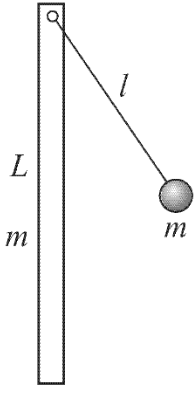
\includegraphics[width=0.17\textwidth]{rodBall.png}
\caption{}
\label{rodBall}
\end{figure}

\begin{ex} %Сив359
Тонкий стержень массы $m$ и длины $L$ (рис. \ref{rodBall}) подвешен за один конец и может вращаться без трения вокруг горизонтальной оси. К той же оси подвешен на нити длины $l$ шарик такой же массы $m$. Шарик отклоняется на некоторый угол и отпускается. При какой длине нити шарик после удара о стержень остановится? Считать удар абсолютно упругим.
\begin{ans}
$l = L/\sqrt{3}$.
\end{ans}
\end{ex}	

\begin{ex}  %Сив359
Каким участком сабли следует рубить лозу, чтобы рука не чувствовала удара? Саблю считать однородной пластинкой.
\begin{ans}
Лозу следует рубить участком сабли, отстоящим на $2/3$ длины от ручки сабли.
\end{ans}
\end{ex}	

\qualProblems

\begin{ex}
Который из следующих объектов обладает наибольшим моментом импульса относительно точки $P$ (рис. \ref{AngularMomentum})? Стрелки указывают на направления вращения и на скорости центров масс дисков, на всех рисунках эти величины имеют одинаковые значения (стрелки равной длины).
\end{ex}	

\begin{figure}[h]
\centering
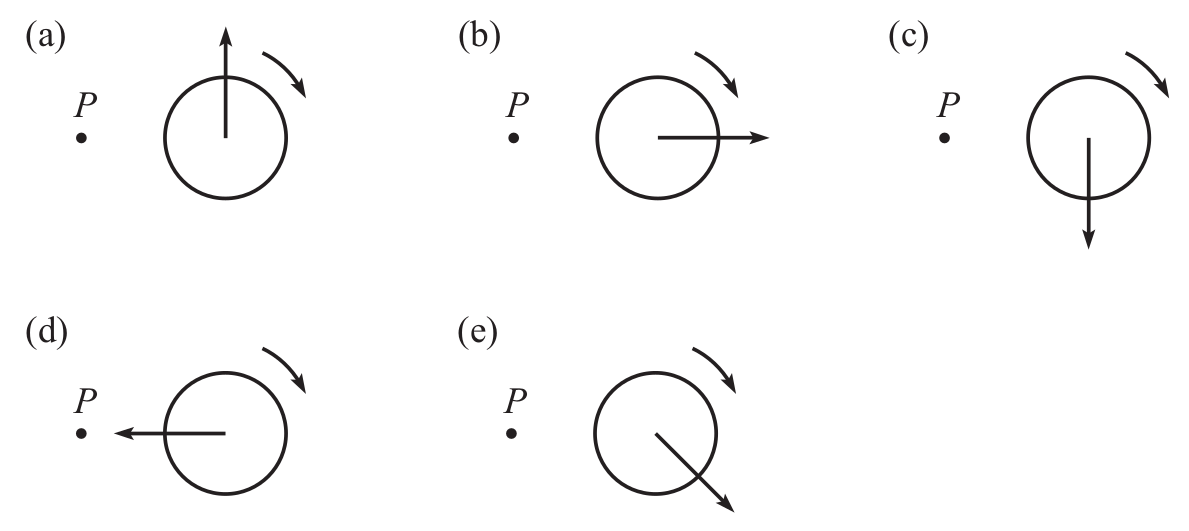
\includegraphics[width=0.8\textwidth]{AngularMomentum.png}
\caption{}
\label{AngularMomentum}
\end{figure}

\begin{ex}
Обладает ли количеством движения (импульсом) однородный диск, вращающийся вокруг своей оси? Ось диска неподвижна.
\end{ex}	

\begin{ex}
Мотоциклист совершает прыжок через колонну автомобилей. Сразу после взлета он заметил, что мотоцикл наклонился немного назад. Если этот наклон сохранится, что у него возникнут проблемы при приземлении, т.к. в тот момент мотоцикл должен быть наклонен немного вперед. Как нужно поступить мотоциклисту, чтобы исправить ситуацию:
\begin{itemize}
\item наклониться вперед;
\item наклониться назад;
\item нажать на газ;
\item нажать на тормоз;
\end{itemize}
\end{ex}	

\begin{ex}
Балерина на льду — вот прекрасный пример, иллюстрирующий закон сохранения момента  импульса. Когда балерина прижимает руки к телу, ее вращение ускоряется именно благодаря сохранению момента импульса (внешние моменты сил при этом отсутствуют). Это, конечно, так, но как объяснить такое явление с точки зрения сил, действующих на балерину,— ведь нам гораздо легче оперировать с силами, чем с моментами импульса. Какая же сила ускоряет вращение балерины?
\end{ex}	


\simpleProblems

\begin{ex}
Тонкий прямой стержень длиной $l = 1$ м прикреплен к горизонтальной оси, проходящей через его конец. Стержень отклонили на угол $\varphi = 60^{\circ}$ от положения равновесия и отпустили. Определить линейную скорость $v$ нижнего конца стержня в момент прохождения через положение равновесия.
\end{ex}	

\begin{ex} %Чертов3.31
Человек стоит на скамье Жуковского и ловит рукой мяч массой $m = 0,4$ кг, летящий в горизонтальном направлении со скоростью $v = 20$ см/с. Траектория мяча проходит на расстоянии $r=0,8$ м от вертикальной оси вращения скамьи. С какой угловой скорость начнет вращаться скамья Жуковского с человеком, поймавшим мяч, если суммарный момент инерции человека и скамьи равен 6 кг$\cdot$м\textsuperscript{2}?
\begin{ans}
$\omega = mvr/(I+mr^2) = 1$ рад/с.
\end{ans}
\end{ex}	

\begin{ex} %Чертов3.45
Кинетическая энергия вращающегося маховика равна 1 кДж. Под действием постоянного тормозящего момента маховик начал вращаться равнозамедленно и, сделав 80 оборотов, остановился. Определите момент силы торможения.
\begin{ans}
$M = E / (2 \pi N) = 2$ Нм.
\end{ans}
\end{ex}	

\begin{ex}
Шарик массой $m = 100$ г, привязанный к концу нити длиной $l_1 = 1$ м, вращается, опираясь на горизонтальную плоскость, с частотой $\nu_1 = 1$ с\textsuperscript{-1}. Нить укорачивается и шарик приближается к оси вращения до расстояния $l_2 = 0.5$ м. С какой частотой $\nu_2$ будет при этом вращаться шарик? Какую работу $A$ совершит внешняя сила, укорачивая нить? Трением шарика о плоскость пренебречь.
\end{ex}	

\begin{ex} %Сив342
Экспериментатор стоит на специальной табуретке и держит в руках вертикальную ось свободно вращающегося колеса, имеющего момент инерции $I_1$ относительно этой оси $AA$ (рис. \ref{hyroscop}). Колесо вращается в горизонтальной плоскости с угловой скоростью $\omega$. Табуретка устроена так, что она может свободно вращаться вокруг вертикальной оси, т. е. представляет собой так называемую скамью Жуковского. Момент инерции табуретки и экспериментатора вокруг вертикальной оси равен $I_2$. Ось колеса и ось табуретки лежат на одной прямой. На какую величину $\Delta E$ изменится кинетическая энергия всей системы табуретки и колеса, если экспериментатор повернет ось колеса на $180^{\circ}$, на $90^{\circ}$?

\begin{figure}[h]
\centering
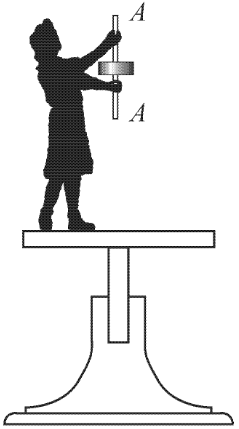
\includegraphics[width=0.25\textwidth]{hyroscop.png}
\caption{}
\label{hyroscop}
\end{figure}

\begin{ans}
1) $\Delta E = 2I_1^2\omega^2/I_2$; 2) $\Delta E = I_1^2\omega^2/2I_2$.
\end{ans}
\end{ex}	

\complexProblems

\begin{ex} %Сив357
Вертикально висящая однородная доска длины $L = 1,5$ м и массы $M = 10$ кг может вращаться вокруг горизонтальной оси, проходящей через ее верхний конец. В нижний конец доски ударяет пуля, летящая горизонтально с начальной скоростью $v_0$ = 600 м/с. Пуля пробивает доску и летит далее со скоростью $v$. Определить скорость $v$, если после выстрела доска стала колебаться с угловой амплитудой $\alpha  = 0,1$ рад. Масса пули $m = 10$ г.
\begin{ans}
$v = v_0 -M/m \sqrt{2gL/3} \sin \alpha /2 = 444$ м/с.
\end{ans}
\end{ex}	


\begin{ex} %Сив343
Монета массы $m$ и радиуса $r$, вращаясь в горизонтальной плоскости вокруг своей геометрической оси с угловой скоростью $\omega$ вертикально падает на горизонтальный диск и «прилипает» к нему. В результате диск приходит во вращение вокруг своей оси. Возникающий при этом момент сил трения в оси диска постоянен и равен $M_0$. Через какое время вращение диска прекратится? Сколько оборотов $N$ сделает диск до полной остановки? Момент инерции диска относительно его геометрической оси $I_0$. Расстояние между осями диска и монеты равно $d$.
\begin{ans}
$t = m\omega r^2 / 2M_0$, $N = M_0t^2/2I$, $I = I_0 + m(d^2 + r^2/2)$.
\end{ans}
\end{ex}	

\begin{ex} %Сив345
На горизонтальный диск, вращающийся вокруг геометрической оси с угловой скоростью $\omega_1$, падает другой диск, вращающийся вокруг той же оси с угловой скоростью $\omega_2$. Моменты инерции дисков относительно указанной оси равны соответственно $I_1$ и $I_2$. Оба диска при ударе сцепляются друг с другом (при помощи острых шипов на их поверхностях). На сколько изменится общая кинетическая энергия вращения системы после падения второго диска? Чем объясняется изменение энергии Геометрические оси обоих дисков являются продолжением одна другой.
\begin{ans}
$\Delta E = I_1 I_2 (\omega_1 - \omega_2)^2/ 2(I_1 + I_2)$.
\end{ans}
\end{ex}	

\begin{figure}[h]
\centering
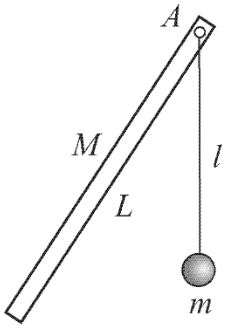
\includegraphics[width=0.22\textwidth]{collisionRod.png}
\caption{}
\label{collisionRod}
\end{figure}

\begin{ex} %Сив358
В общей точке подвеса $A$ (рис. \ref{collisionRod}) подвешены шарик на нити длины $l$ и однородный стержень длины $L$, отклоненный в сторону на некоторый угол. При возвращении стержня в положение равновесия происходит упругий удар. При каком соотношении между массами стержня $M$ и шарика $m$ шарик и точка удара стержня будут двигаться после удара с равными скоростями
в противоположных направлениях? При каком соотношении между
массами $M$ и $m$ описанный процесс невозможен?
\begin{ans}
$ML^2 = ml^2$, при $M \leq m$.
\end{ans}
\end{ex}	

\begin{ex} %Сив348
Однородный диск $A$ массы $M_1$ и радиуса $r_1$ (рис. \ref{2Disks}) раскручен до угловой скорости $\omega_0$ и приведен в контакт с диском $B$, ось вращения которого перпендикулярна к оси диска $A$. Масса диска $B$ равна $M_2$, а расстояние между точкой соприкосновения и осью диска $A$ равно $a$. Найти установившиеся угловые скорости дисков $\omega_1$ и $\omega_2$ и потерю энергии в процессе установления. Трением в осях, а также трением качения пренебречь.

\begin{figure}[h]
\centering
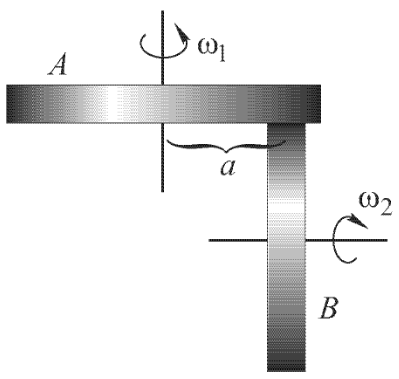
\includegraphics[width=0.4\textwidth]{2Disks.png}
\caption{}
\label{2Disks}
\end{figure}

\begin{ans}
$\omega_1 = \frac{M_1r_1^2\omega_0}{M_1r_1^2 + M_2a^2}$, $\omega_2 = \frac{M_1r_1^2 a \omega_0}{(M_1r_1^2 + M_2a^2)r_2}$, $\Delta E = \frac{M_1 M_2r_1^2a^2\omega_0^2}{4(M_1r_1^2 + M_2a^2)}$.
\end{ans}
\end{ex}	

\begin{ex} %Сив354

\begin{figure}[h]
\centering
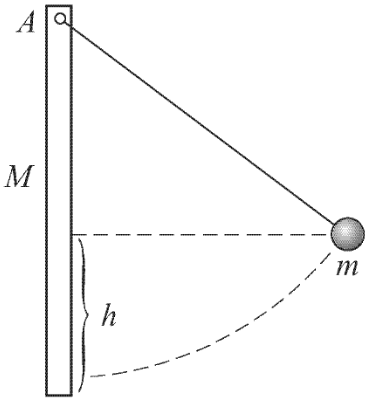
\includegraphics[width=0.3\textwidth]{rodOscil.png}
\caption{}
\label{rodOscil}
\end{figure}

Математический маятник массы $m$ и стержень массы $M$ (рис. \ref{rodOscil}) подвешены к одной и той же точке $A$, вокруг которой они могут свободно колебаться. Длина нити маятника равна длине стержня. Шарик маятника отклоняют в сторону, так что он приподнимается на высоту $h$ относительно своего нижнего положения. Затем шарик отпускают, и он сталкивается неупруго со стержнем. Как будут двигаться шарик и нижний конец стержня после удара и на какие высоты они поднимутся? Как изменится ответ задачи, если первоначально нижний конец стержня был поднят на высоту $h$?
\begin{ans}
После удара шарик и стержень будут подниматься как единое тело на высоту $h = \frac{6m^2}{(M+2m)(M+3m)}H$.
\end{ans}
\end{ex}	

\begin{ex} %Сив344
Сплошной однородный короткий цилиндр радиуса $r$, вращающийся вокруг своей геометрической оси с частотой $\nu$ об/с, ставят в вертикальном положении на горизонтальную поверхность. Сколько оборотов $N$ сделает цилиндр, прежде чем вращение его полностью прекратится? Коэффициент трения скольжения между основанием цилиндра и поверхностью, на которую он поставлен, не зависит от скорости вращения и равен $\mu$.
\begin{ans}
$N = 2\pi r n^2/(4 \mu g)$.
\end{ans}
\end{ex}	

\clearpage